\documentclass[12pt]{article}
\usepackage[utf8]{inputenc}
\usepackage[T2A]{fontenc}
\usepackage[english, russian]{babel}
\usepackage{graphicx, float, multicol, hyperref, pgfplots}

\graphicspath{{pictures/}}

\title{Лабораторная работа 1.3.1 \\
       Определение модуля Юнга на основе исследования деформаций растяжения и изгиба}
\author{Балдин Виктор Б01-303}

\begin{document}
    \maketitle

    \section{Aннотация}
    \par \textbf{Цель работы:} экспериментально получить зависимость между напряжением и деформацией
    для двух простейших напряженных состояний упругих тел: одностороннего сжатия и чистого изгиба;
    по результатам эксперимента вычислить модул Юнга.\\
    \par \noindent \textbf{В работе используются:} в первой части - прибор Лермантова, проволока
    из исследуемого материала,
     зрительная трубка со шкалой,
    набор грузов, микрометр, рулетка;  во второй части - стойка для изгибания балки, индикатор для
    измерения величин прогиба,
набор исследуемых стержней, грузы, линейка, штангенциркуль.

    \section{Определение модуля Юнга по измерениям растяжения проволоки}
    \subsection{Теоретические сведения}
    Растяжение проволоки соответствует напряженному состоянию вдоль одной оси, которое описывается формулой:
\begin{equation}
    \frac{F}{S} = E \frac{\Delta l}{l}
    \label{lermantov}
\end{equation}
    Эту формулу можно переписать также в следующем виде:
    \begin{equation}
        F = k\Delta l,
    \end{equation}
    где $k = ES / l$ -- жесткость проволоки.
    Измерения производятся на установке Лермантова.
    Направим зрительную трубку на зеркальце.
    Выведем формулу для расчета растяжения длины проволоки по показаниям шкалы
    прибора (см. рис. 1).
    Так как мы считаем проволоку слабо растяжимой, справедлива оценка $\Delta l \ll r$, где
    $r$ -- длина рычага. С учетом этого, угол наклона зеркальца к горизонтали можно
    найти как $\alpha = \Delta l/r$. С другой стороны, из соображений геометрической оптики
    угол $\alpha$ можно найти как угол между продолжениями соответствующих лучей:
    \begin{equation}
        \alpha = \frac{n}{2h},
    \end{equation}
    где $n$ -- показания шкалы, $h$ -- расстояние от шкалы до
    зеркальца.
    \par Таким образом, удлинение проволоки можно выразить как:
    \begin{equation}
        \Delta l = n\frac{r}{2h}
        \label{dlina}
    \end{equation}

    Отсюда формулу (1) можно переписать как
    \begin{equation}
        F = \frac{ESr}{2lh}n
    \end{equation}

    \subsection{Методика измерений}
    \par Для определения модуля Юнга используется прибор Лермонтова,
    схема которого изображена на рис. 1. Верхний конец проволоки П, изготовленной
    из исследуемого материала, прикреплен к консоли К, а
    нижний -- к цилиндру, которым оканчивается шарнирный кронштейн
    Ш. На этот же цилиндр опирается рычаг $r$, связанный с зеркальцем
    3. Таким образом, удлинение проволоки можно измерить по углу
    поворота зеркальца.\\
    \par Натяжение проволоки можно менять перекладыванием грузов
    с площадки О на площадку М, не меняя при этом нагрузку на кронштейн,
    и, как следствие, его деформацию.

    \begin{figure}[H]
        \centering
        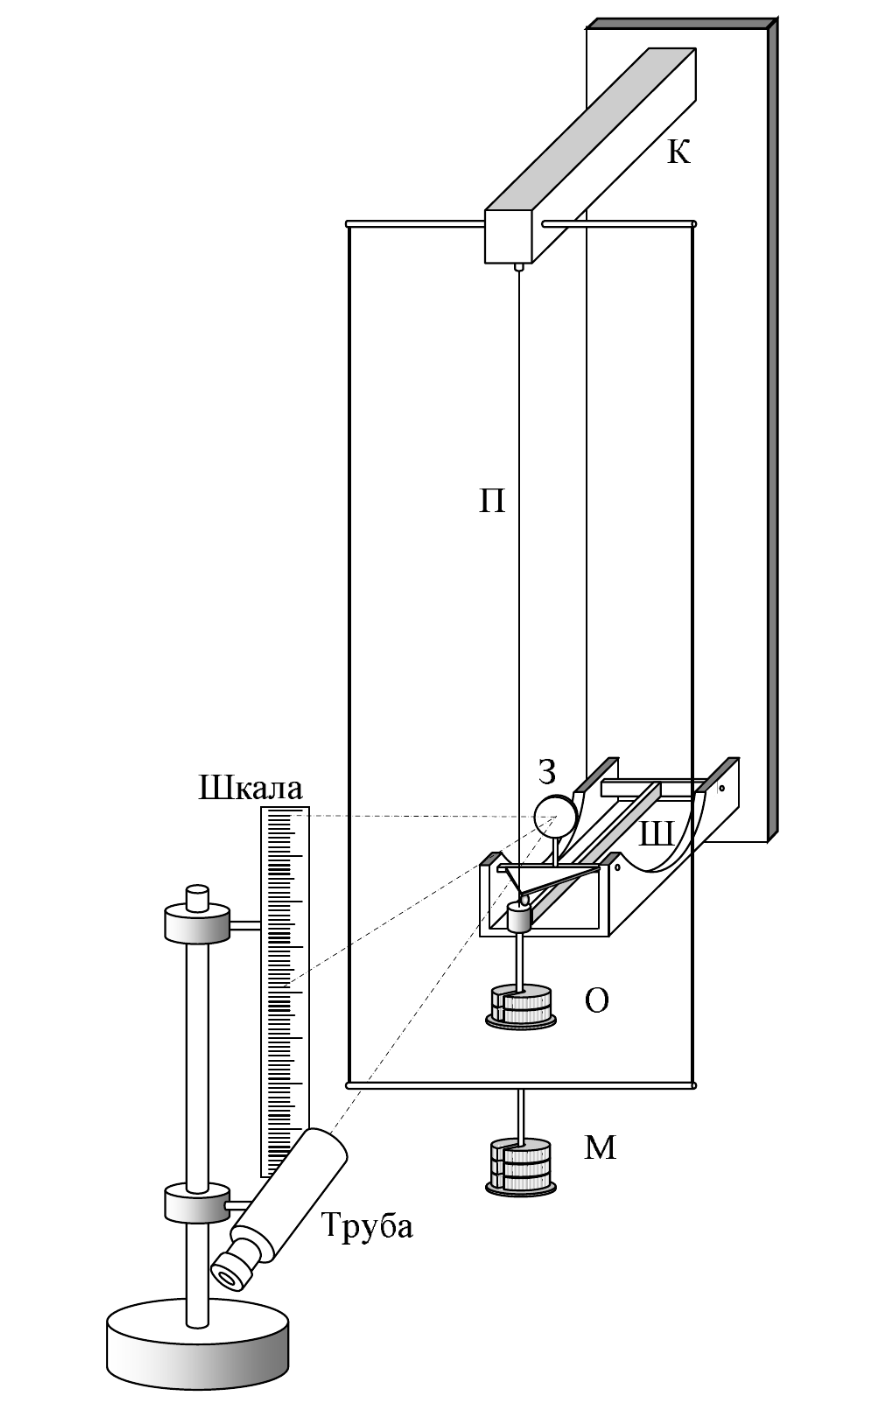
\includegraphics[scale = 0.3]{pictures/lermantov.png}
        \caption{Прибор Лермантова}
    \end{figure}

    \subsection{Используемое оборудование}
    Параметры используемого оборудования представим в таблице:
    \begin{table}[H]
        \centering
        \caption{Оборудование}
        \begin{tabular}{|c|c|}
        \hline
        Прибор         & Точность \\ \hline
        Штангенциркуль & $\pm 0.05$ мм \\ \hline
        Индикатор      & $\pm 0.01$ мм \\ \hline
        Рулетка        & $\pm 5$ мм \\ \hline
        Линейка        & $\pm 0.5$ мм \\ \hline
        Прибор Лермантова & $\pm 1$ мм \\ \hline
        \end{tabular}
    \end{table}


    \subsection{Результаты измерений и обработка данных}
    \begin{enumerate}
    \item Сведем характеристики установки в таблицу:
    \begin{table}[H]
        \centering
        \caption{Параметры прибора Лермантова}
        \begin{tabular}{|c|c|c|c|c|}
        \hline
        $d_{\tiny{\mbox{пр}}}$, мм & $r$, мм & $l$, см & $h$, см & $\sigma_{\tiny{\mbox{пр}}}$, Н/мм$^2$\\ \hline
        $0.46 \pm 0.01$            & $15 \pm 1$ & $177.6 \pm 0.5$  & $144.0\pm 0.05$   & 900\\ \hline
        \end{tabular}
    \end{table}
    \item Оценим, сколько грузов можно подвесить к проволоке. Для этого найдем площадь
    сечения проволоки и погрешность: \[S = \frac{\pi d^2}{4} = 0.17\;\mbox{мм}^2,\]
    \[\sigma_S = 2S\frac{\sigma_d}{d} = 0.01\;\mbox{мм}^2\]
    Предельная нагрузка на разрушение:
    \[ P_{max} = 0.3\sigma_{\mbox{\tiny{пр}}}S = 45,9\; \mbox{Н},\]
    \[ \sigma_{P_{max}} = 2.7\; \mbox{Н} \]
    Согласно полученному значению, можно подвесить все грузы.
    \item Теперь проверим предыдущую оценку на практике. Для этого будем подвешивать
    каждый раз на 1 груз больше и следить при помощи шкалы прибора, чтобы проволока
    возвращалась в исходное состояние. На практике деформация была замечена уже после
    подвешивания первых 6 грузов.
    \item Перейдем к измерениям. Будем последовательно класть одни и те же грузы,
    потом поочередно их снимать по принципу стека. Проведем этот цикл 2 раза:
    \begin{table}[H]
    \centering
    \caption{Зависимость показаний шкалы от нагрузки}
    \begin{tabular}{|c|c|c|c|c|c|}
    \hline
    $\Delta m$, гр & $P$, Н & $n_1 \downarrow$, см & $n_1\uparrow$, см & $n_2 \downarrow$, см & $n_2 \uparrow$, см \\ \hline
    501.4          & 4.9    & 13.5                 & 15.8              & 15.8                 & 15.2               \\ \hline
    245.6          & 7.3    & 16.1                 & 18.7              & 18.9                 & 18.4               \\ \hline
    245.3          & 9.7    & 18.6                 & 21.6              & 21.3                 & 21.3               \\ \hline
    245.6          & 12.1   & 21.8                 & 23.9              & 24.2                 & 24.1               \\ \hline
    245.5          & 14.5   & 24.4                 & 26.5              & 26.8                 & 26.8               \\ \hline
    \end{tabular}
    \end{table}
    \item Построим графики зависимости $F(n)$ для первого и второго эксперимента.
    \end{enumerate}

    \section{Определение модуля Юнга по измерениям изгиба балки}
    \subsection{Теоретические сведения}
    Модуль Юнга материала стержня $E$ связан с величиной
    прогиба $y_{max}$ как:
    \begin{equation}\label{balka}
        E=\frac{Pl^3}{4ab^3y_{max}}
    \end{equation}
    где $P$ - нагрузка на стержень, $l$ - расстояние меду точками опоры,
    $a$ - ширина балки, $b$ - высота балки.

    \subsection{Экспериментальная установка}
    \par Экспериментальная установка состоит из прочной стойки с
    опорными призмами А и Б (рис. 2). На ребра призм опирается исследуемый
    стержень В. В середине стержня на призме Д подвешена площадка
    П с грузами. Измерять величину
    прогиба можно с помощью индикатора И, укрепляемого
    на отдельной штанге. Полный оборот большой
    стрелки индикатора соответствует 1 мм и одному делению малого циферблата.
    \begin{figure}[H]
        \centering
        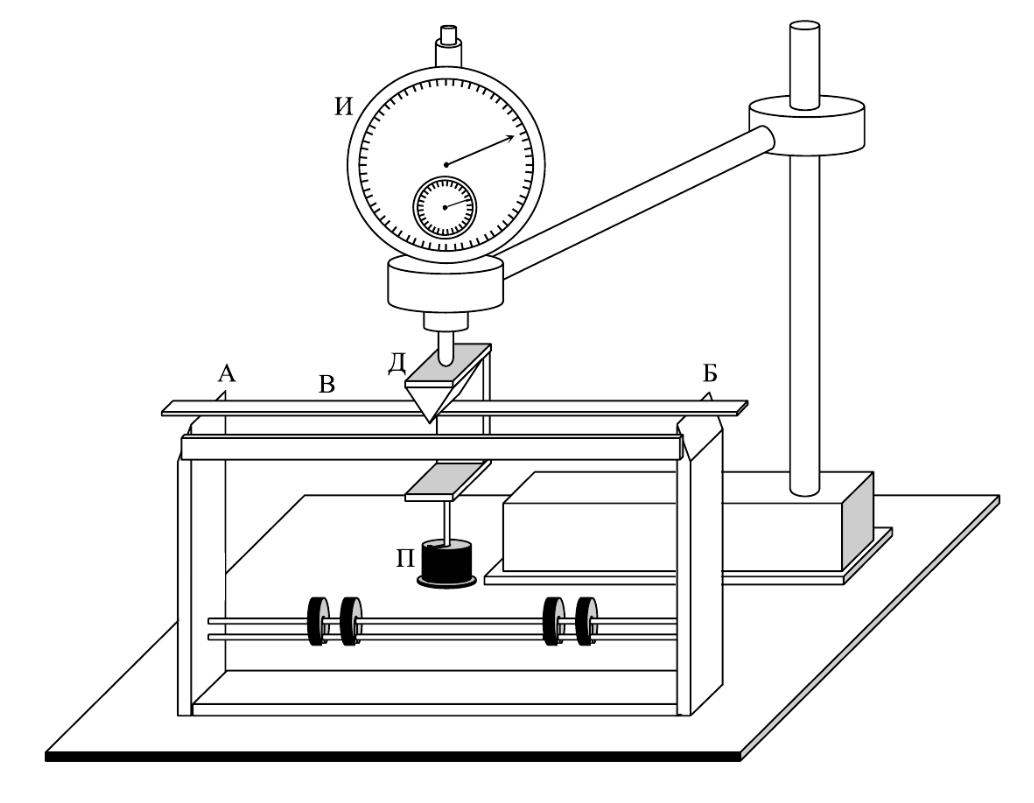
\includegraphics[scale = 0.25]{pictures/balka.png}
        \caption{Схема установки для измерения модуля Юнга}
    \end{figure}

    \subsection{Используемое оборудование}
    Линейка, штангенциркуль для измерения параметров установки;
    индикатор для измерения стрелы прогиба.
    \par Для уменьшения погрешности вследствие прогиба стола
    при изменении нагрузки на стержень, грузы перед началом эксперимента
    лучше расположить на рейке над нижней полкой опорной стойки.

\end{document}
